% $Header: /cvsroot/latex-beamer/latex-beamer/examples/beamerexample1.tex,v 1.47 2004/11/04 15:43:51 tantau Exp $

\documentclass{beamer}
%\documentclass{article}
%\usepackage[envcountsect]{beamerarticle}

% Do NOT take this file as a template for your own talks. Use a file
% in the directory solutions instead. They are much better suited.

% Try the class options [notes], [notes=only], [trans], [handout],
% [red], [compress], [draft] and see what happens!

% Copyright 2003 by Till Tantau <tantau@users.sourceforge.net>.
%
% This program can be redistributed and/or modified under the terms
% of the LaTeX Project Public License Distributed from CTAN
% archives in directory macros/latex/base/lppl.txt.

% For a green structure color use:
%\colorlet{structure}{green!50!black}

\usepackage{array,paralist}
\usepackage{tabularx}
\usepackage{eurosym}

\mode<article> % only for the article version
{
  \usepackage{fullpage}
  \usepackage{hyperref}
}


\mode<presentation>
{
  \setbeamertemplate{background canvas}[vertical shading][bottom=red!10,top=blue!10]

  \usetheme{CambridgeUS}
  \usefonttheme[onlysmall]{structurebold}
}

%\setbeamercolor{math text}{fg=green!50!black}
%\setbeamercolor{normal text in math text}{parent=math text}

\usepackage{amsmath,amssymb}
\usepackage[latin1]{inputenc}
\usepackage{colortbl}
\usepackage[english]{babel}

%\usepackage{lmodern}
%\usepackage[T1]{fontenc} 

\usepackage{times}
\setbeamercovered{dynamic}

%% Titel etc
\title[Patienten unter Strom: Mein erstes EKG]{Eine kurze Einf�hrung in die biomedizinische Me�technik}
\author[Noe]{Marcel Noe}
\institute[TNG]{
        \inst{}TNG Technology Consulting GmbH}
\date[2012]


%% Hauptseite
\begin{document}
\frame{\titlepage}

\section<presentation>*{Einf�hrung}

\begin{frame}
  \frametitle{�berblick}
  \tableofcontents[part=1,hidesubsections]
\end{frame}

\part<presentation>{Vortrag}


\logo{}
\section{Einf�hrung}
\subsection{Motivation}
\begin{frame}
    \frametitle{Biomedizinische Technik}

    \begin{columns}[T]
        \begin{column}{5cm}
            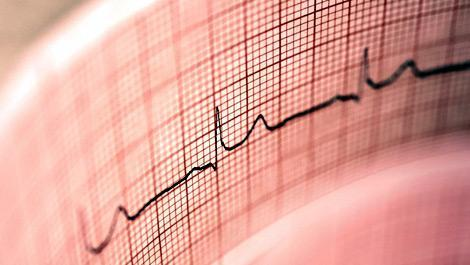
\includegraphics[width=5cm]{images/ekg_fancy.jpg}\\
            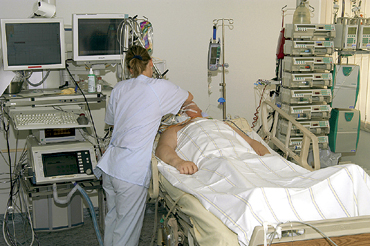
\includegraphics[width=5cm]{images/its.jpg}\\
        \end{column}

        \begin{column}{7cm}
            \begin{itemize}
                \item Patienten �berwachen 
                \item Krankheiten diagnostizieren
                \item Leben retten
            \end{itemize}
        \end{column}
    \end{columns}
\end{frame}

\section{Medizinische Grundlagen}
\subsection{Anatomie des Menschen: Nerven}
\begin{frame}
    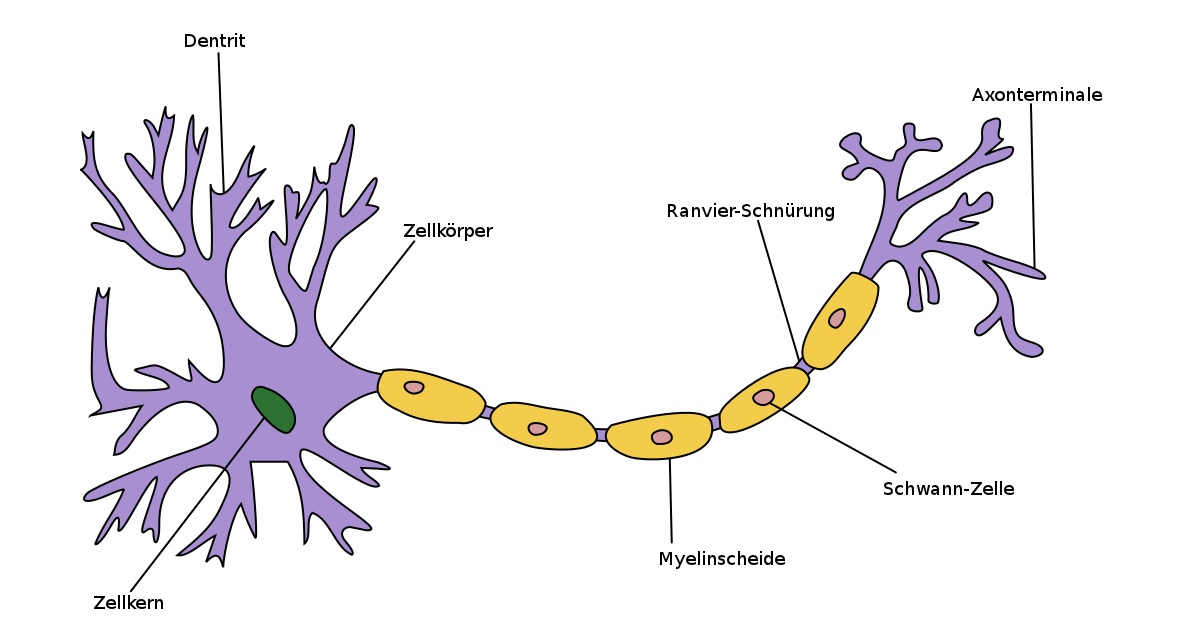
\includegraphics[width=12cm]{images/Neuron_Hand-tuned-text.jpg}
\end{frame}

\begin{frame}
    \begin{center}
        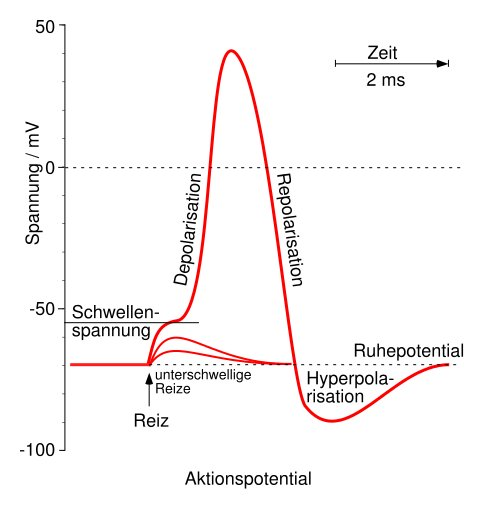
\includegraphics[height=8cm]{images/Aktionspotential.jpg}
    \end{center}
\end{frame}

\begin{frame}
    \begin{center}
        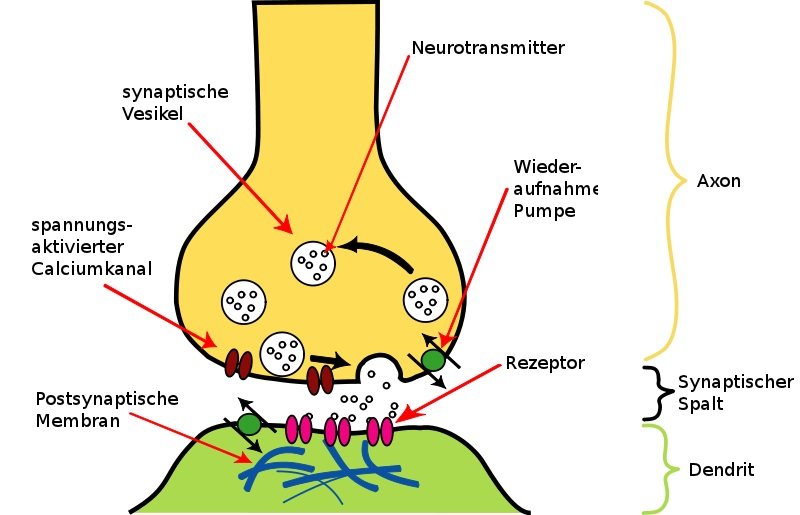
\includegraphics[height=7.5cm]{images/synaptischer_spalt.jpg}
    \end{center}
\end{frame}


\subsection{Anatomie des Menschen: Blutgef��e}
\begin{frame}
    \begin{center}
        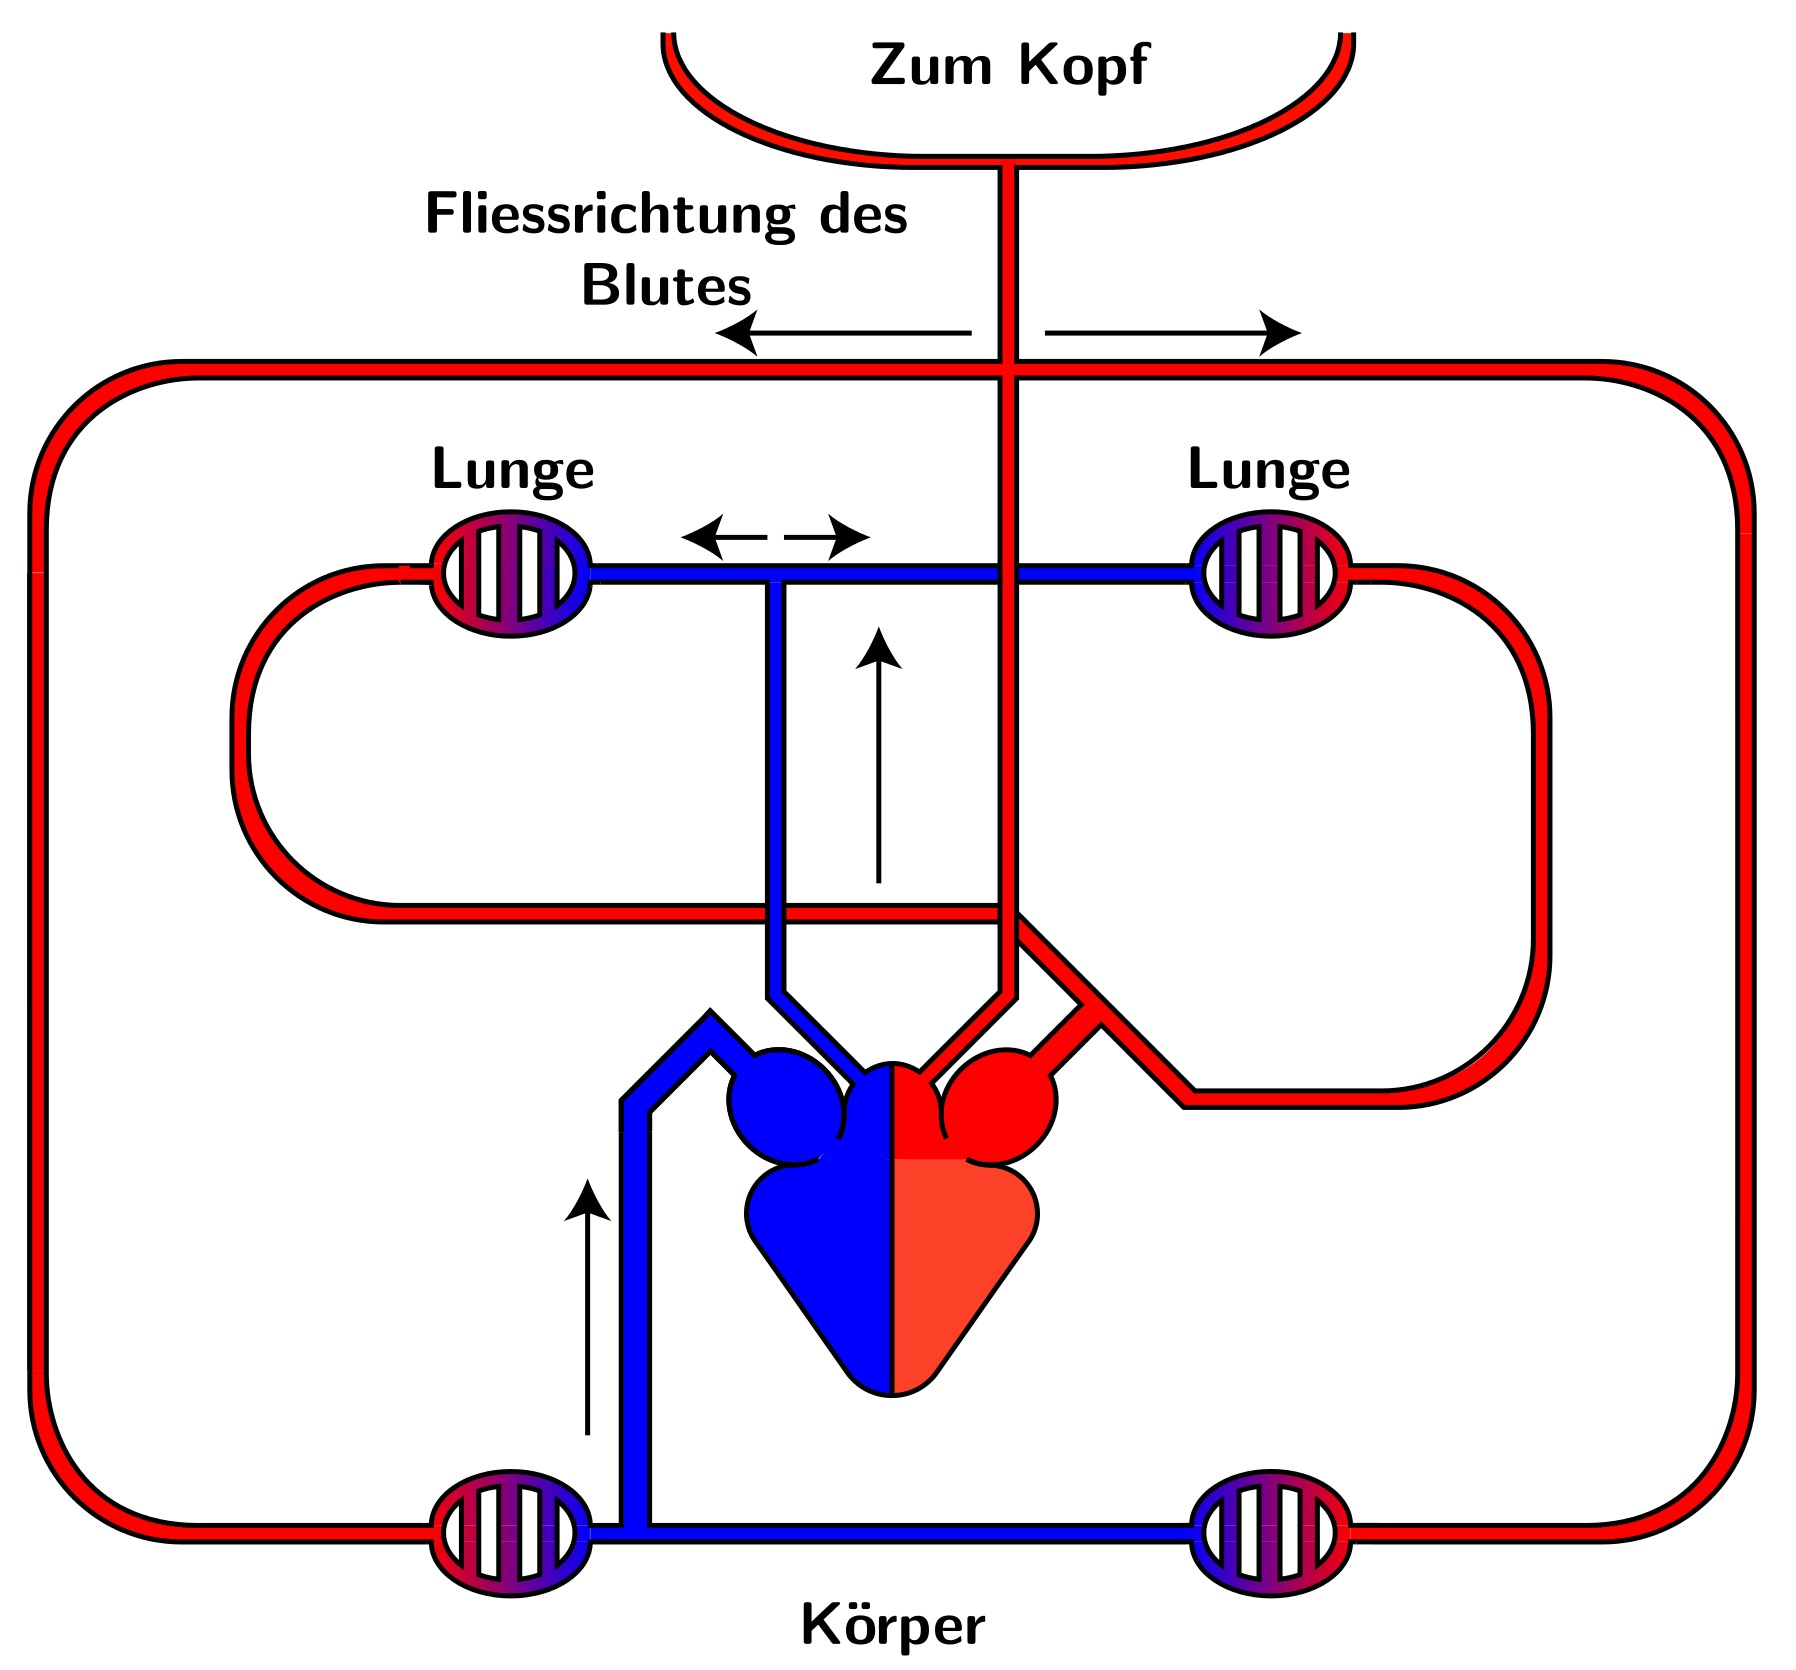
\includegraphics[height=7.5cm]{images/blutkreislauf.jpg}
    \end{center}
\end{frame}

\subsection{Anatomie des Menschen: Herz}
\begin{frame}
    \begin{center}
        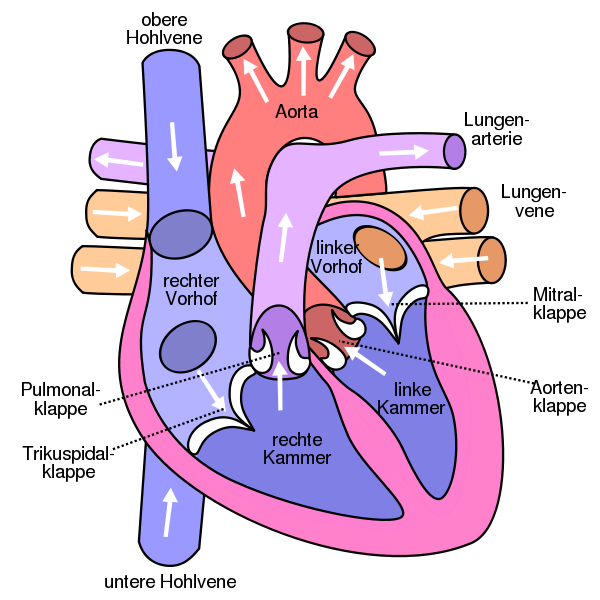
\includegraphics[height=7.5cm]{images/herz.png}
    \end{center}
\end{frame}

\begin{frame}

    \begin{columns}
        \begin{column}{5cm}
            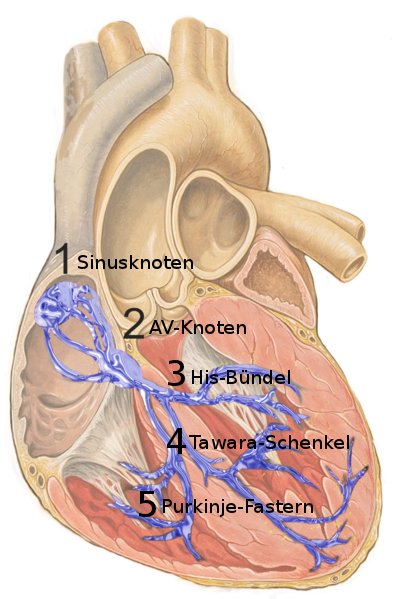
\includegraphics[height=7.5cm]{images/reizleitungssystem.png}
        \end{column}

        \begin{column}{7cm}
            \begin{itemize}
                \item Spontane Depolarisation:
                \item Sinusknoten: 40-200 Schl�ge pro Minute 
                \item AV-Knoten: 40-50 Schl�ge pro Minute
                \item His-B�ndel: 20-30 Schl�ge pro Minute
            \end{itemize}
        \end{column}
    \end{columns}

\end{frame}


\section{Messtechnik}
\subsection{Ableitung von elektrischen Signalen}
\begin{frame}
    \frametitle{Ein- und Auskopplung elektrischer Signale}
    \begin{alertblock}{Problem: Reizweiterleitung im K�rper basiert auf Ionenleitung.}
        Natrium, Kalium, Calcium, Magnesium, Chlorid, Phosphat und Hydrogencarbonat 
    \end{alertblock}
    \begin{exampleblock}{L�sung: Verwendung entsprechender Elektroden.}
        % Quelle: seniorenland.de
        \begin{figure}
            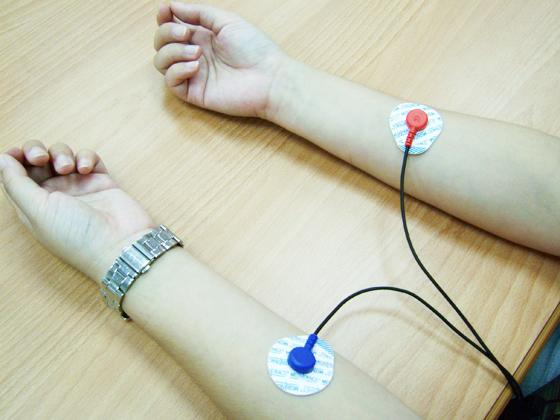
\includegraphics[height=4cm]{images/elektroden.jpg}
            \hspace{0.5cm}
            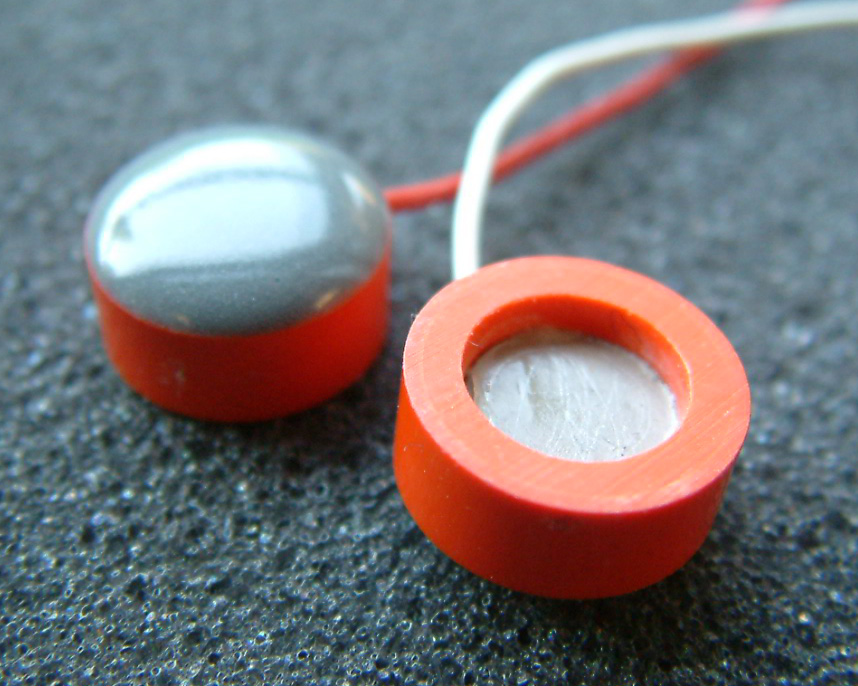
\includegraphics[height=4cm]{images/electrodes2.jpg}
        \end{figure}
    \end{exampleblock}
\end{frame}

\begin{frame}
    \frametitle{Instrumentierungsverst�rker}
    \begin{center}
        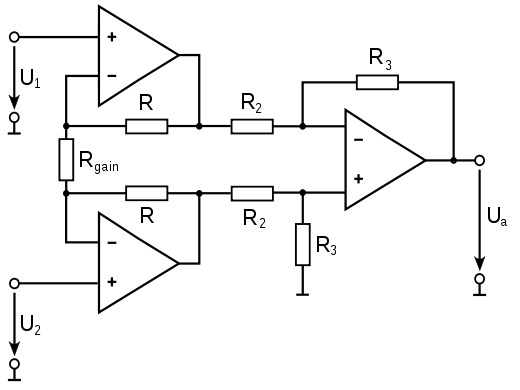
\includegraphics[height=6cm]{images/instrumentierungsverstaerker.png}
    \end{center}
\end{frame}


\begin{frame}
    \frametitle{St�rsignale}
    \begin{columns}
        \begin{column}{6cm}
            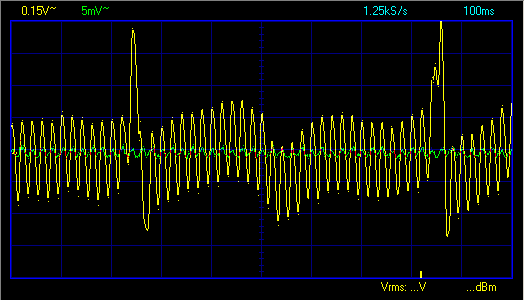
\includegraphics[height=3.5cm]{images/ekg_multimeter1.png}
        \end{column}

        \begin{column}{6cm}
            \begin{itemize}
                \item "50Hz Brummen"
                \item Kapazitive Einkopplung (Ungl�cklicherweise direkt in den Patienten \\$\rightarrow$ Schirmung wirkungslos)
                \item Unzureichend gegl�ttete Versorgungsspannung \\$\rightarrow$ Batterien, Kondensatorgl�ttung, Galvanische Trennung

                \item Induktive Einkopplung\\$\rightarrow$ Schirmung
            \end{itemize}
        \end{column}
    \end{columns}
\end{frame}

\begin{frame}
    \frametitle{Behandlung von St�rsignalen}
    \begin{exampleblock}{Vorschlag: Erdung des Patienten}
        Durch die Erdung des Patienten wird ein gemeinsames Bezugspotenzial zwischen 
        Patient und Messger�t hergestellt. St�rsignale werden symmetrisch eingekoppelt
        und verschwinden somit.
    \end{exampleblock}

    \begin{alertblock}{Problem: Gef�hrlich!}
        Im Falle eines Kurzschlusses k�nnen hohe Str�me durch den Patienten flie�en.
        $\rightarrow{}$ Potenziell t�dlich und daher mittlerweile verboten.\\
        Fr�her jedoch oft angewendet.
    \end{alertblock}
\end{frame}

\begin{frame}
    \frametitle{Behandlung von St�rsignalen}
    \begin{exampleblock}{Bezugspotentialsteuerung (Driven right leg)}
        Das St�rsignal wird in der Messchaltung abgeleitet und invertiert an den
        Patienten zur�ckgegeben. \\
        $\rightarrow{}$ St�rung und Gegensignal heben sich gegenseitig auf.
        
        % Source: ti.com
        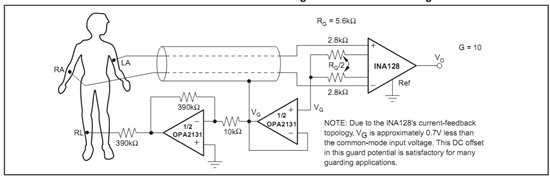
\includegraphics[width=12cm]{images/legdrive.jpg} 
    \end{exampleblock}
\end{frame}

\begin{frame}
    \frametitle{Behandlung von St�rsignalen}
     \begin{exampleblock}{Ausfiltern des 50Hz St�rsignals mit einem Notchfilter}
        Mit Hilfe einer Bandsperre mit einer Sperrfrequenz von 50Hz wird das 
        St�rsignal ausgefiltert.
        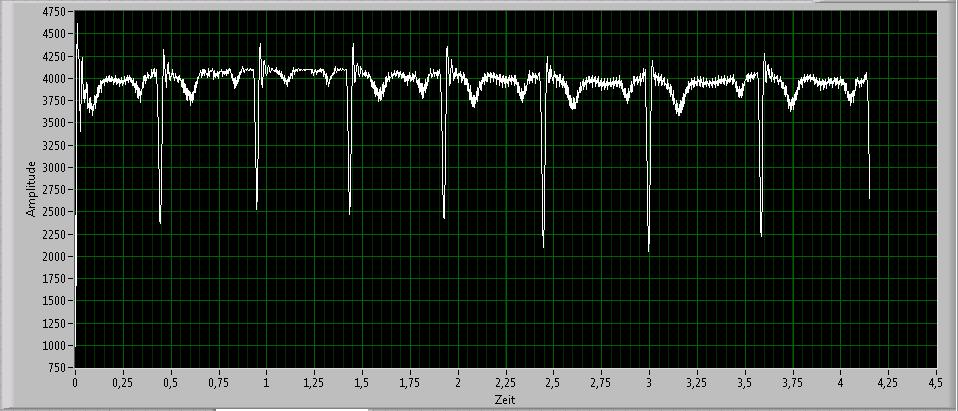
\includegraphics[width=12cm]{images/filter_notch.jpg}
     \end{exampleblock}

\end{frame}


\begin{frame}
    \frametitle{Behandlung von St�rsignalen}
     \begin{exampleblock}{Hochpa�filter}
        Ausfilterung von Signalen mit einer Frequenz von �ber 50Hz. 
        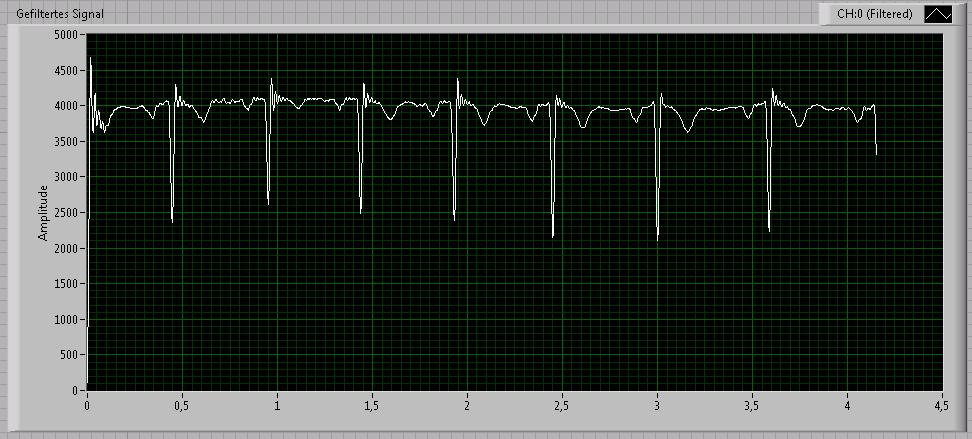
\includegraphics[width=12cm]{images/abtastrate_300.jpg}
     \end{exampleblock}
\end{frame}

\section{Ger�te}
\subsection{Das EKG}
\begin{frame}
    \frametitle{Ein Standard-EKG}
    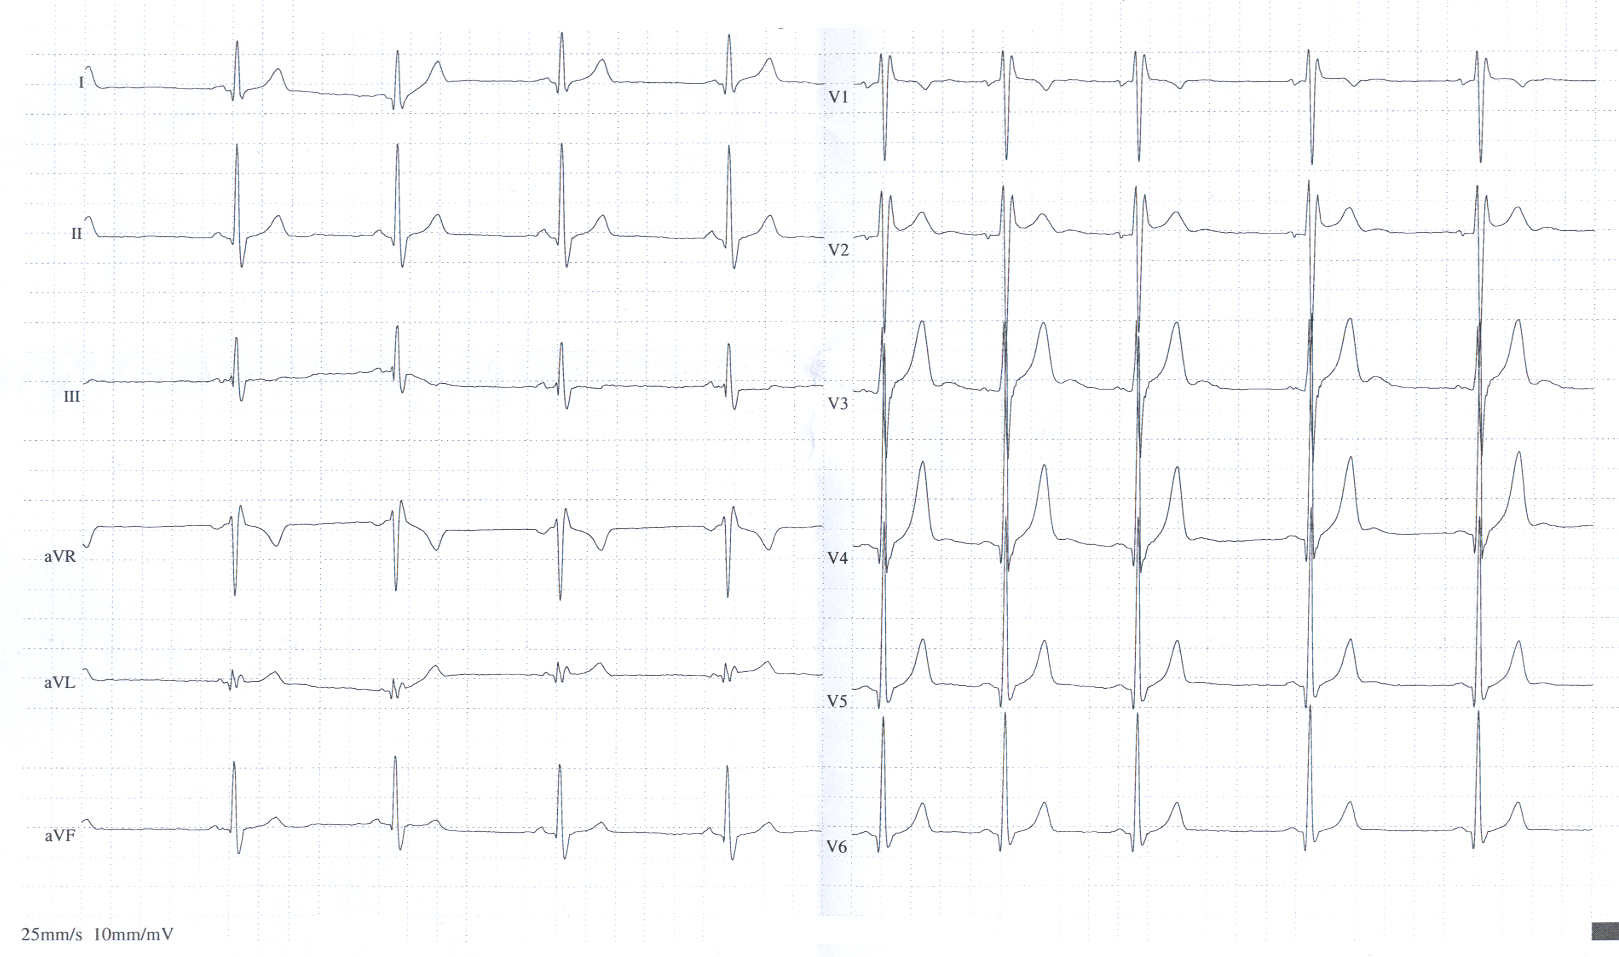
\includegraphics[width=12cm]{images/ekg2.jpg}
\end{frame}

\begin{frame}
    \frametitle{EKG-Komplex}
    \begin{center}
        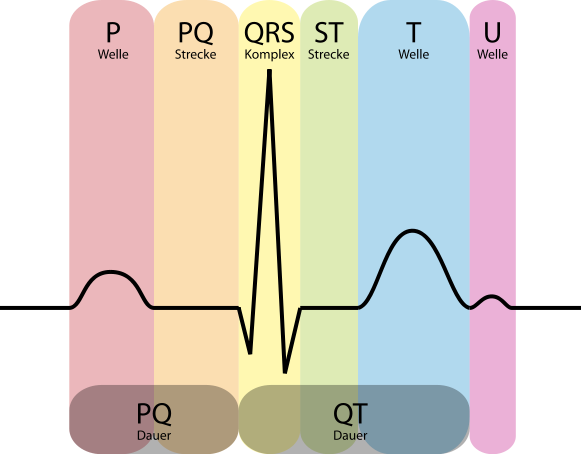
\includegraphics[width=8cm]{images/ekg_komplex.png}
    \end{center}
\end{frame}

\begin{frame}
    \frametitle{Bedeutung des EKGs}
    % Source: Netdoktor.de
    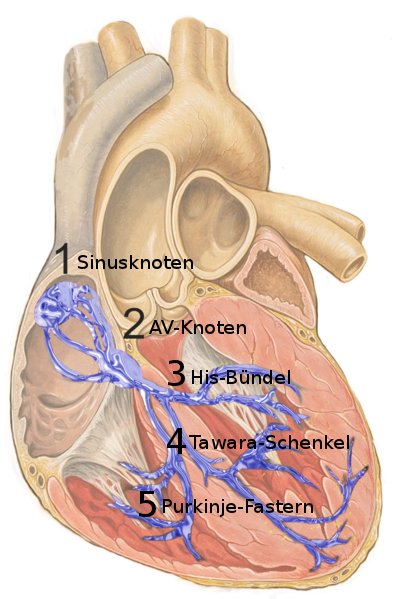
\includegraphics[height=7.5cm]{images/reizleitungssystem.png}
    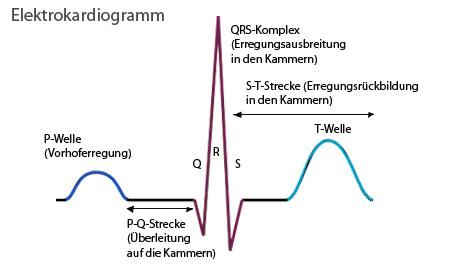
\includegraphics[width=7.5cm]{images/ekg_bedeutung.jpg}
\end{frame}

\begin{frame}
    \frametitle{Positionierung der Elektroden}

    \begin{columns}[T]
        \begin{column}{5cm}
            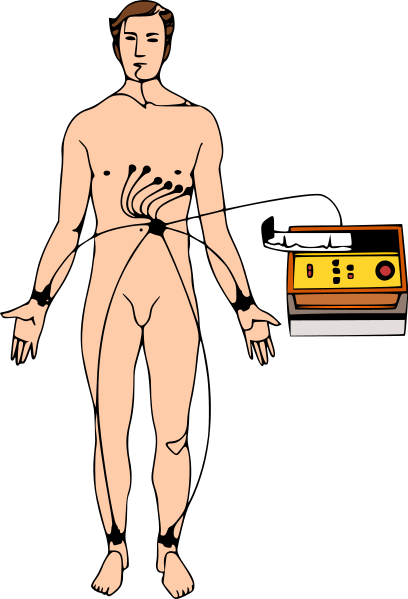
\includegraphics[height=7.5cm]{images/ableitung.png}
        \end{column}

        \begin{column}{7cm}
            \begin{itemize}
                \item 12 Kan�le:
                \item Einthoven I, II, III (Extremit�ten)
                \item Goldberger aVR, aVL, aVF (Extremit�ten)
                \item Wilson V1-V6 (Brustwand)
            \end{itemize}
        \end{column}
    \end{columns}

\end{frame}

\begin{frame}
    \frametitle{Schaltung eines einfachen EKG-Verst�rkers}
    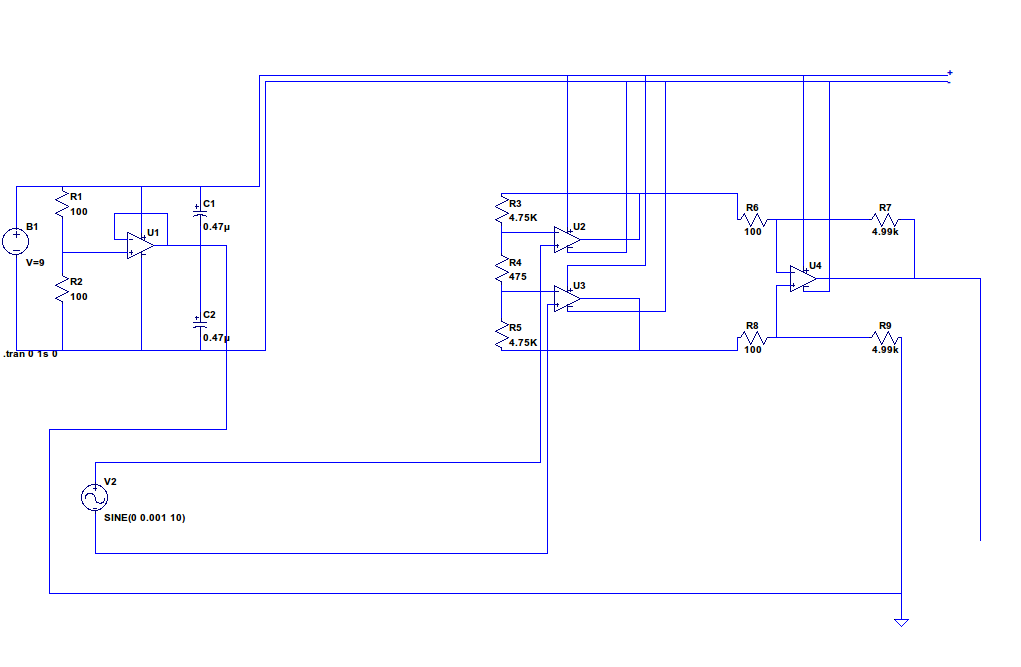
\includegraphics[height=8cm]{images/ekg_schaltung.png}
\end{frame}

\begin{frame}
    \frametitle{Schaltung eines einfachen EKG-Verst�rkers}
    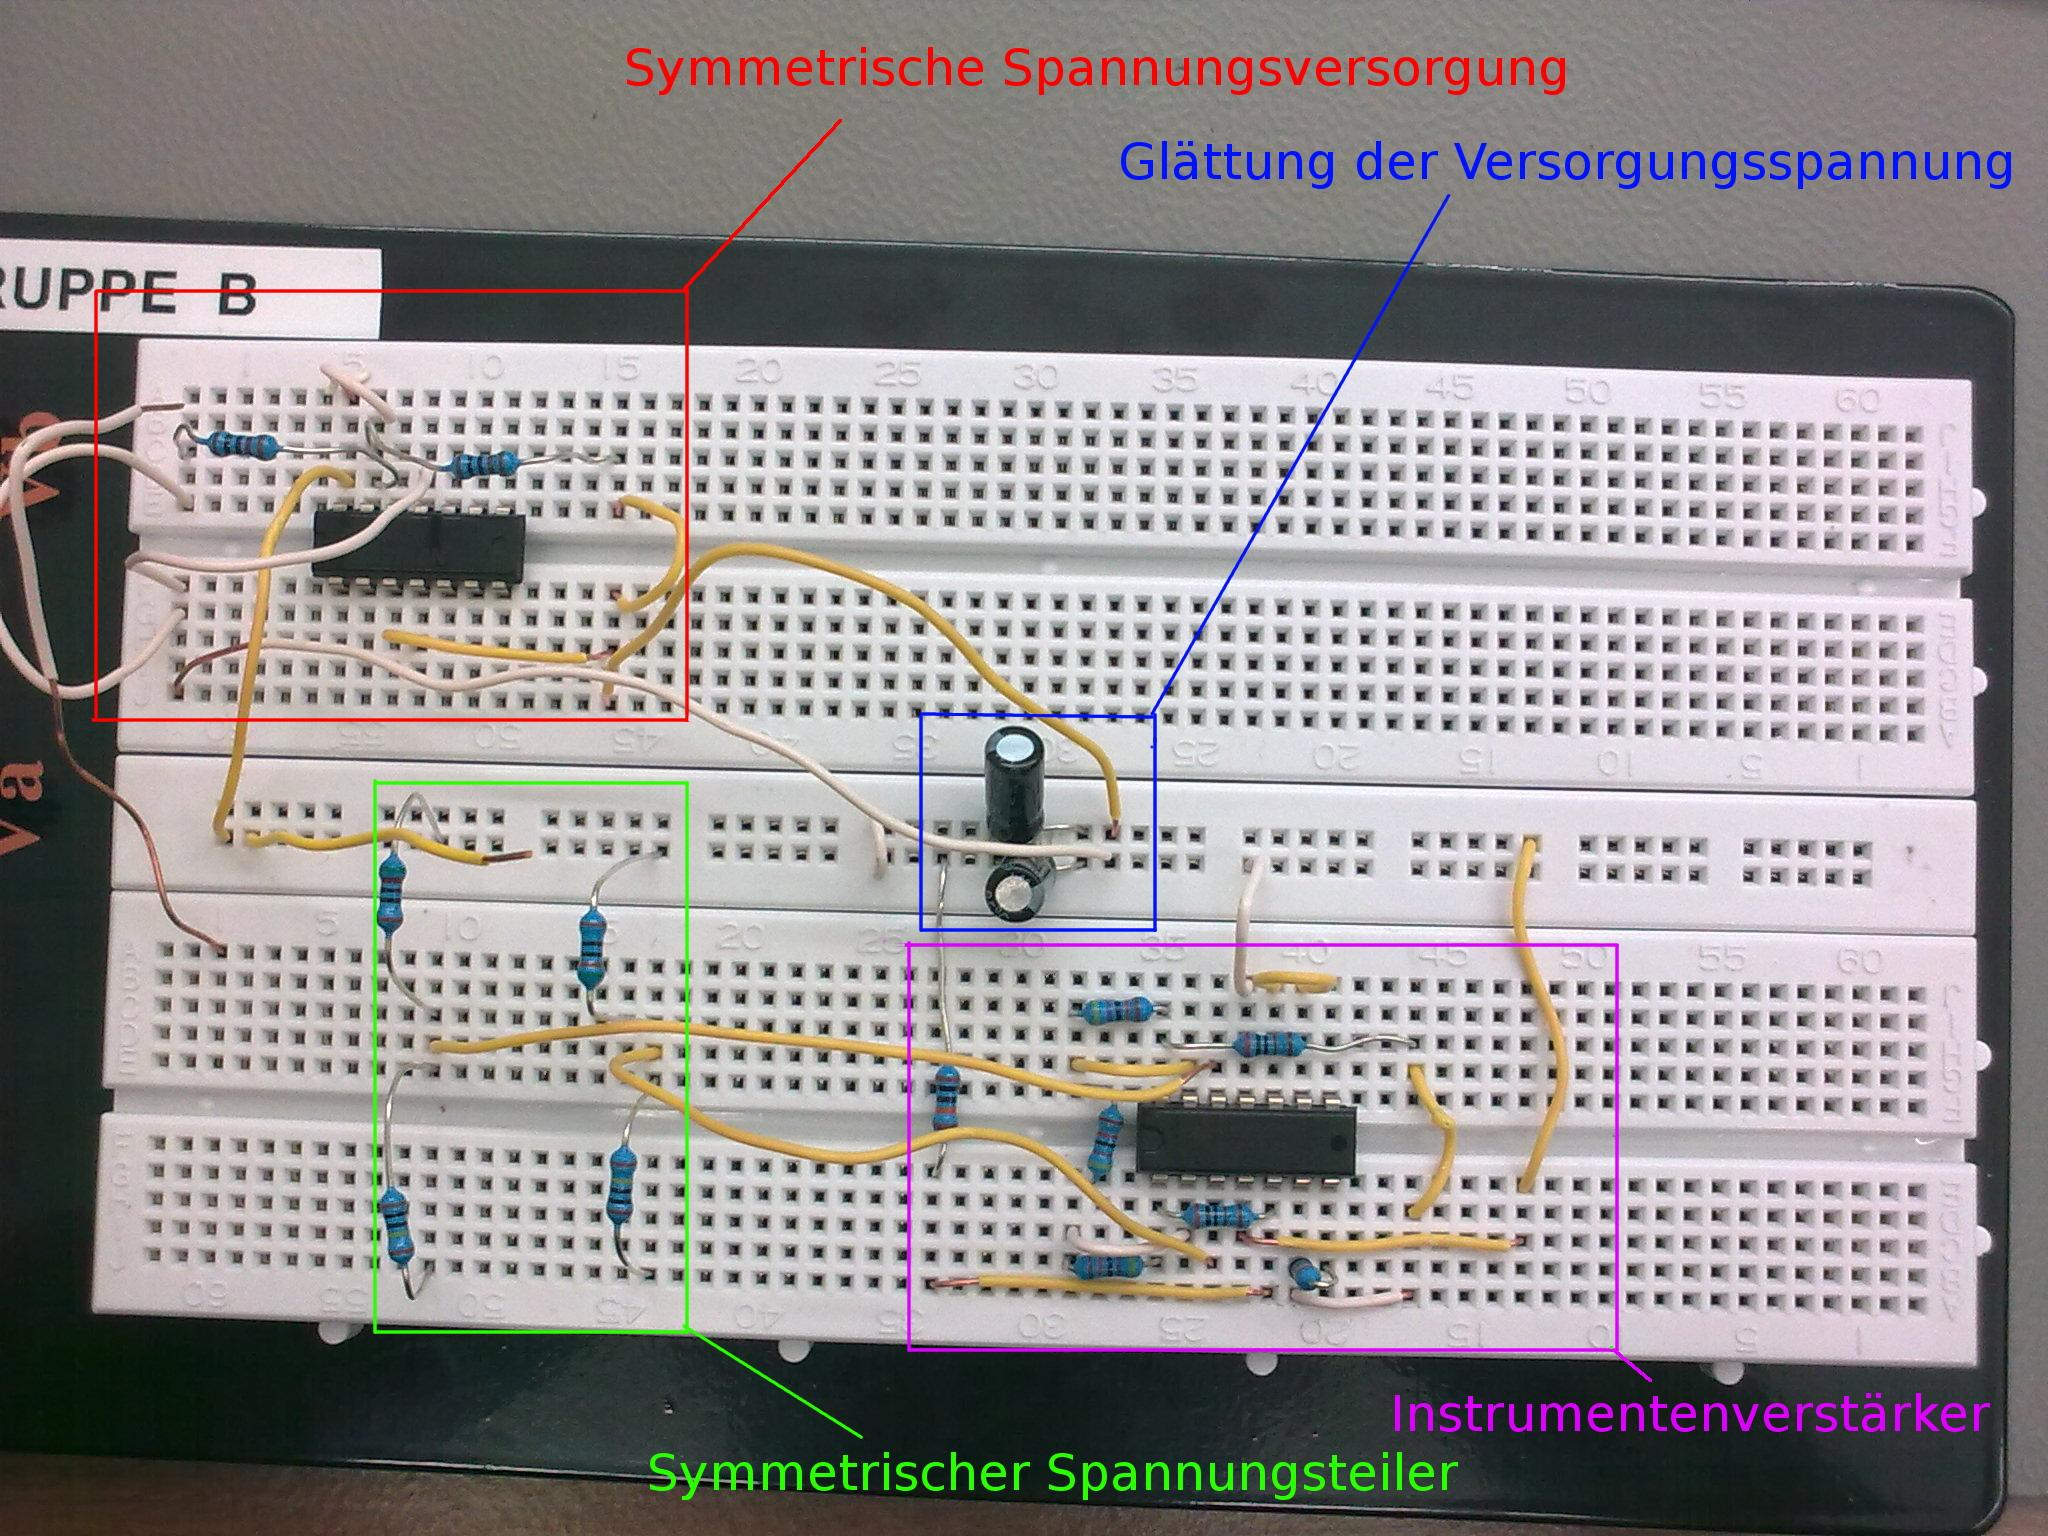
\includegraphics[height=7cm]{images/ekg_steckbrett.png}
\end{frame}

\subsection{Defibrillator}
\begin{frame}
    \frametitle{Das Kammerflimmern}
    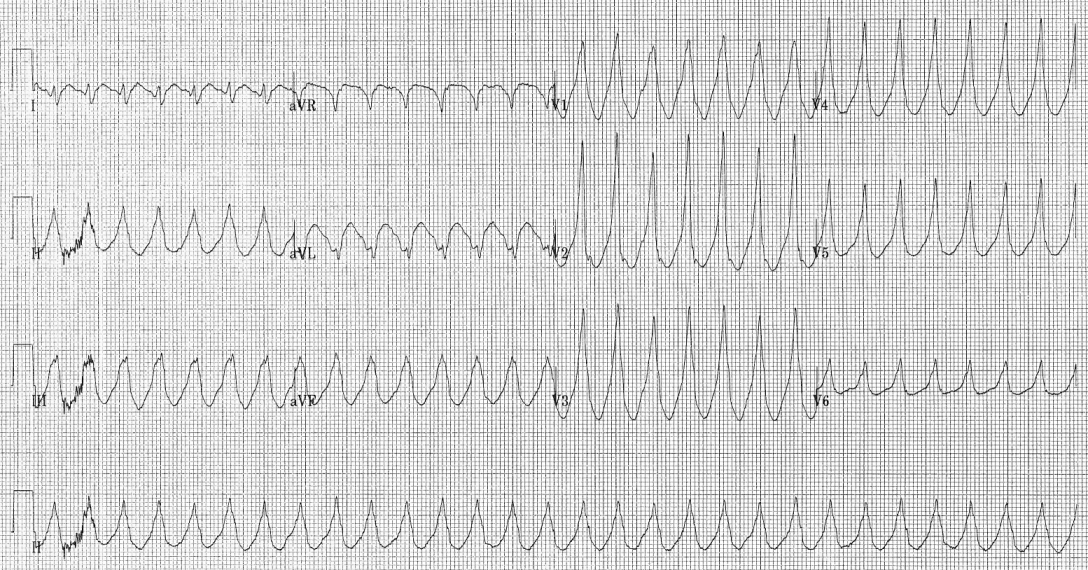
\includegraphics[height=6cm]{images/vtach.png}
\end{frame}

\begin{frame}
    \frametitle{Ursache des Kammerflimmerns}
    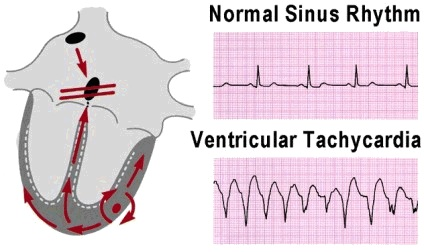
\includegraphics[height=6cm]{images/vtach2.jpg}
\end{frame}

\begin{frame}
    \frametitle{Der Defibrillator}
    \begin{figure}
        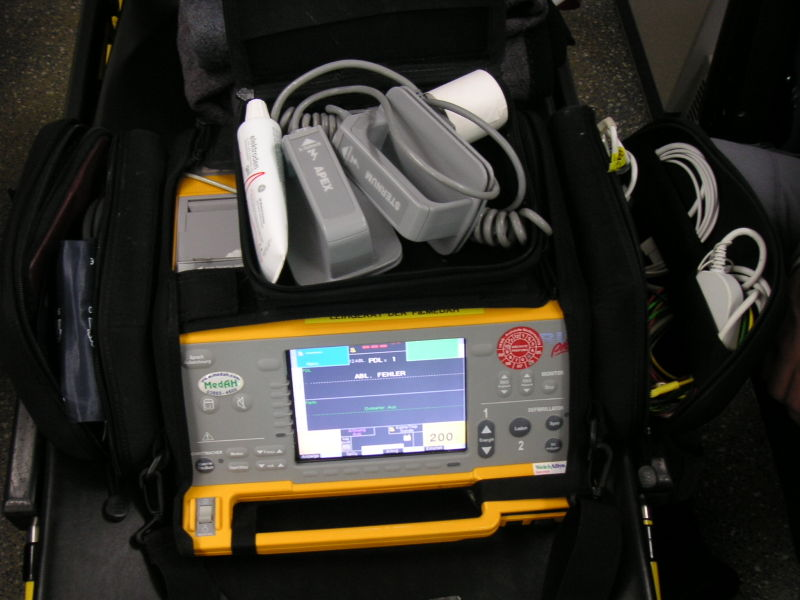
\includegraphics[height=4.2cm]{images/defi.jpg}
        \hspace{0.5cm}
        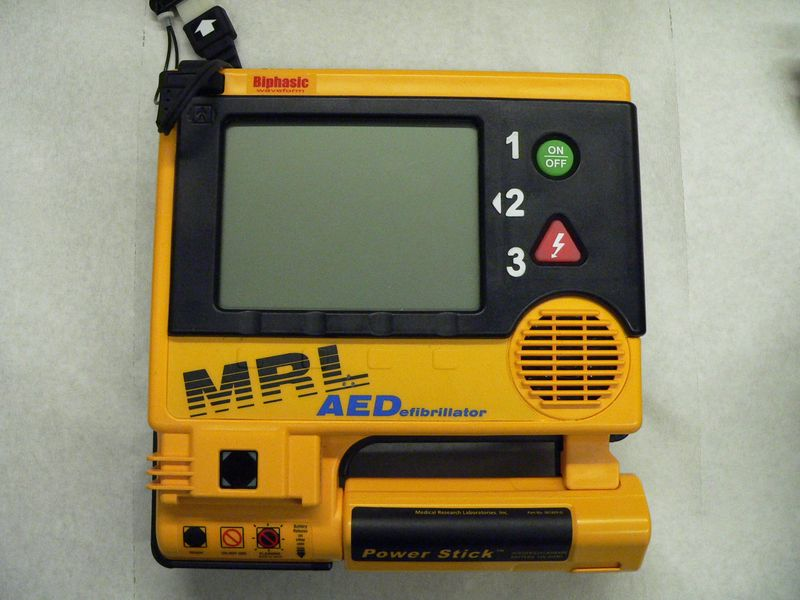
\includegraphics[height=4.2cm]{images/aed.jpg}
    \end{figure}
\end{frame}

\begin{frame}
    \frametitle{Biphasischer Schock} 

    \begin{columns}[T]
        \begin{column}{6cm}
            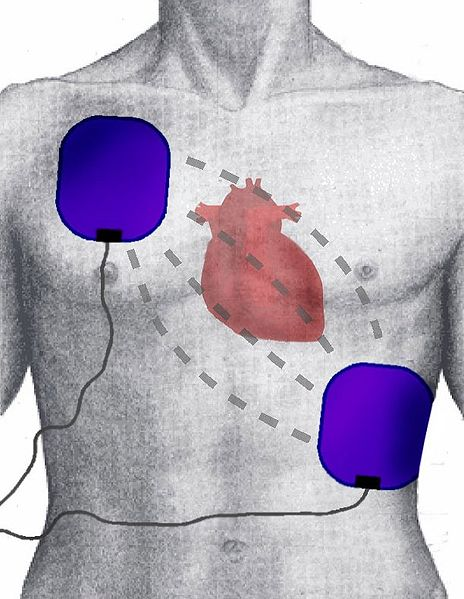
\includegraphics[width=5.5cm]{images/electrode_position.jpg}    
        \end{column}

        \begin{column}{7cm}
            \begin{itemize}
                \item 150-360 Joule 
                \item 1,5 Ampere 
                \item 750 Volt 
                \item Depolarisierung von �ber 70\% des Myokards
            \end{itemize}
            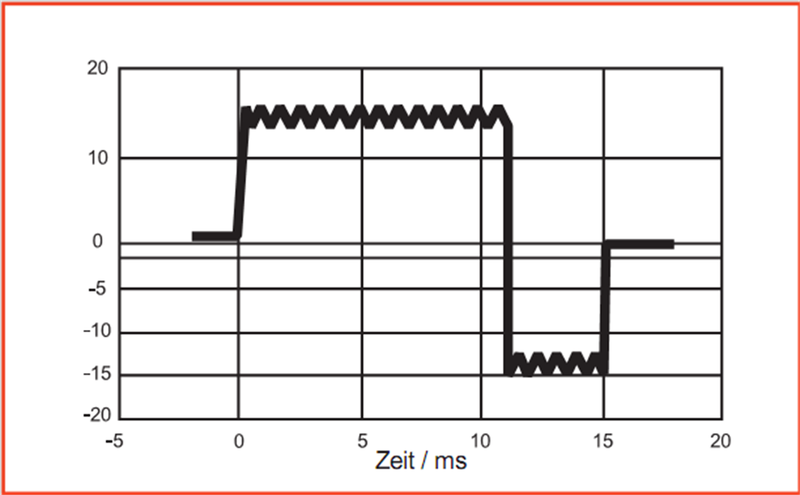
\includegraphics[width=5.5cm]{images/shock.png}
        \end{column}
    \end{columns}
\end{frame}

\begin{frame}
    \frametitle{Defi-Schaltung} 
    \begin{center}
        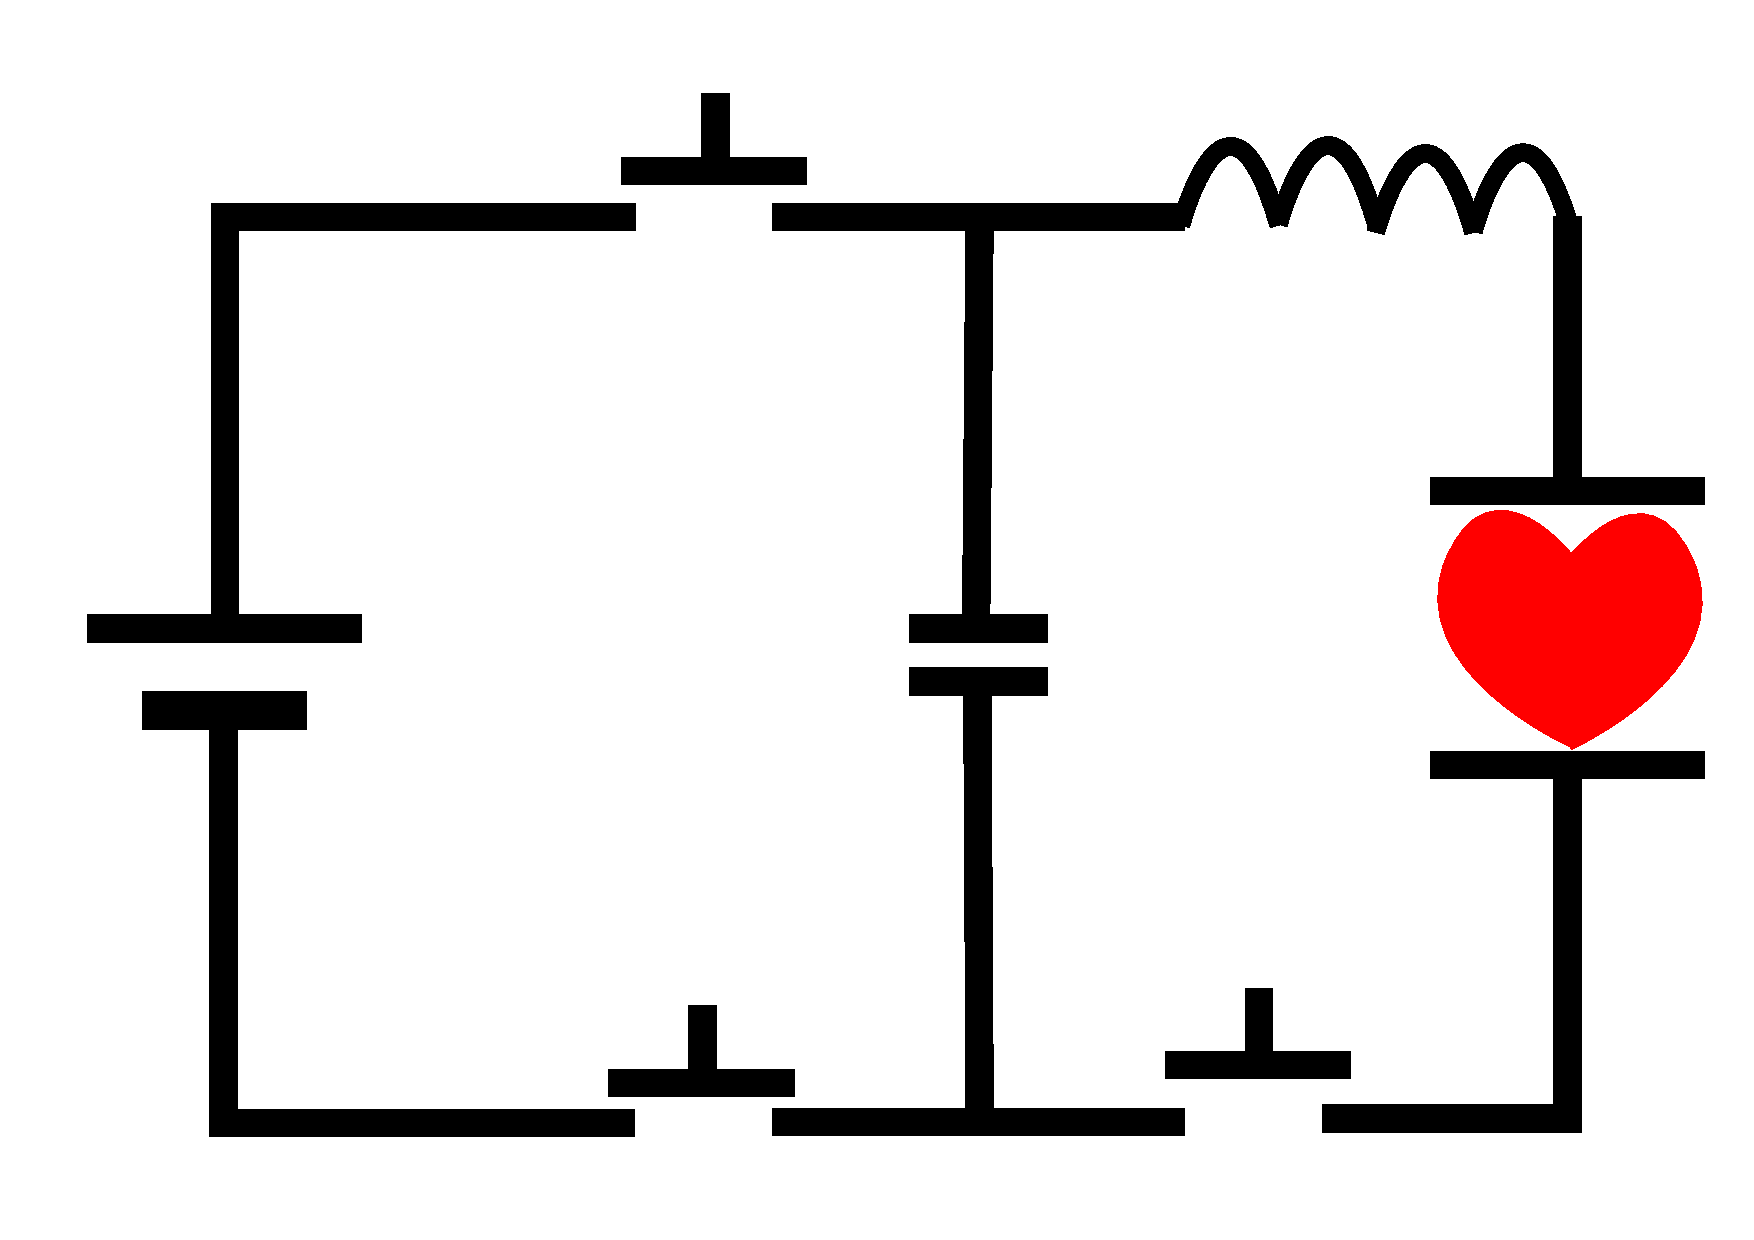
\includegraphics[width=10cm]{images/defib.pdf}
    \end{center}
\end{frame}

\subsection{Herzschrittmacher}
\begin{frame}
    \frametitle{AV-Block}
    \begin{columns}[T]
        \begin{column}{6cm}
            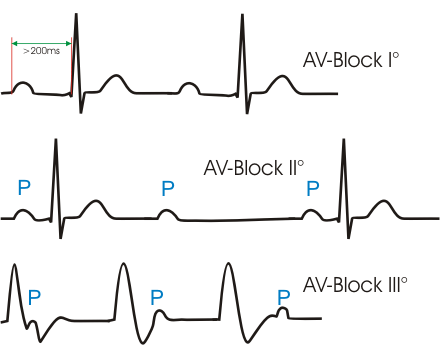
\includegraphics[width=6cm]{images/avb.png}
        \end{column}

        \begin{column}{7cm}
            \begin{itemize}
                \item 1. Grad: Erregungsleitung verz�gert 
                \item 2. Grad: 2:1, 3:1 oder 4:1 Block 
                \item 3. Grad: Keine �bertragung mehr zwischen Vorhof und Kammern 
            \end{itemize}
        \end{column}
    \end{columns}
\end{frame}

\begin{frame}

    % http://www.apotheken-umschau.de
    \begin{figure}
        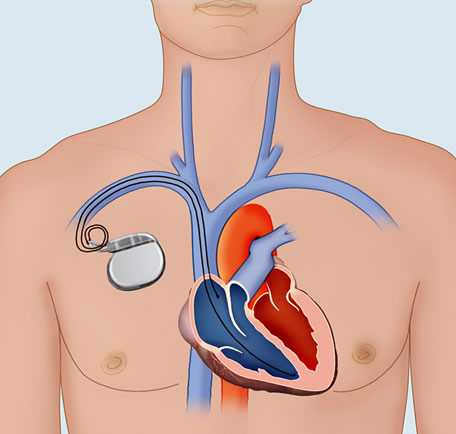
\includegraphics[height=5.5cm]{images/schrittmacher3.jpg}
        \hspace{0.5cm}
        % http://www.kardiodoc-zieger.de/
        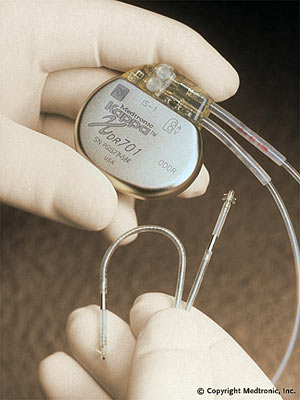
\includegraphics[height=5.5cm]{images/schrittmacher2.jpg}
    \end{figure}

    \begin{table}
        \begin{scriptsize}
        \begin{tabular}{|l|l|l|l|l|}
             \hline
             1. & 2. & 3. & 4. & 5. \\
             \hline
             Stimulationsort & Registrierungsort & Betriebsart & Frequenzadaption & Multifokal \\
             \hline
             0 (keiner) & 0 (keiner) & 0 (keine) & 0 (keine) & 0 (keine) \\
             A (Atrium) & A (Atrium) & T (getriggert) & R (adaptiv) & A (atrium) \\
             V (Ventrikel) & V (Ventrikel) & I (Inhibiert) & & V (Ventrikel) \\
             D (Dual A+V) & D (Dual A+V) & D (Dual T+I) & & D (Dual A+V) \\
             S (Single A/V) & S (Single A/V) & & & \\
             \hline
        \end{tabular}
        \end{scriptsize}
    \end{table}
\end{frame}

\begin{frame}
   \frametitle{Impulsgenerator eines Herzschrittmachers}
   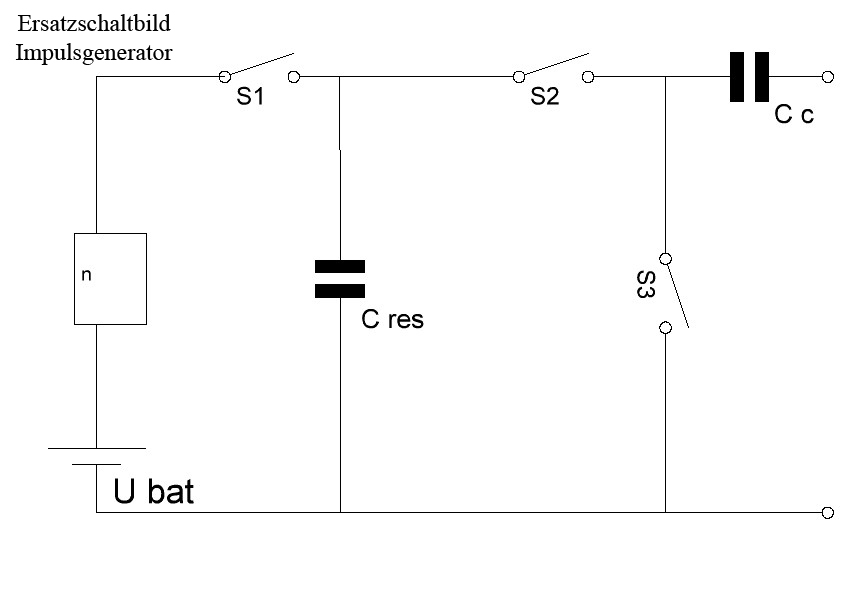
\includegraphics[width=10cm]{images/impulsgenerator.jpg}
\end{frame}


\begin{frame}
    \frametitle{Herzschrittmacher Elektroden}
    % http://www.info-kt.de/
    \begin{figure}
        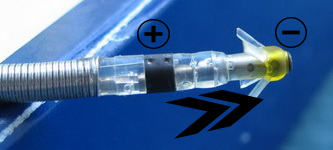
\includegraphics[width=5.2cm]{images/elektrode1.png}
        \hspace{0.5cm}
        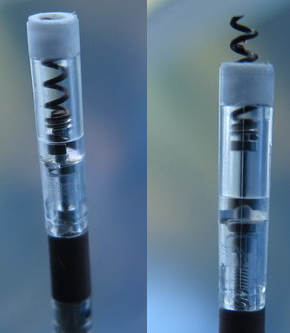
\includegraphics[width=5.2cm]{images/elektrode2.png}
    \end{figure}
\end{frame}

\begin{frame}
    \frametitle{Fraktale Elektroden}
    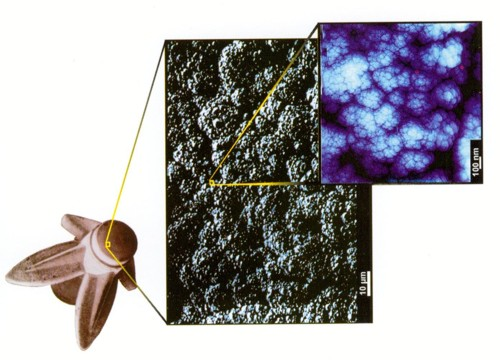
\includegraphics[width=8cm]{images/fractal2.jpg}
\end{frame}

\subsection{Fragen}
\begin{frame}
    \frametitle{Fragen?}

    \begin{center}
        
\includegraphics[height=6cm]{fragezeichen.jpg}
    \end{center}
\end{frame}
\end{document}
